\section{GUI and interaction design}

\subsection{User Interface}
\label{sec:gui_ui}

In the following we have included screenshots for some of the most
important parts of our user interface. All data shown is our test
data, has been randomly generated, so many people share the same
image, have strange titles, projects and department names.

\subsubsection{Employee List}

\begin{figure}[H]
    \centerline{ 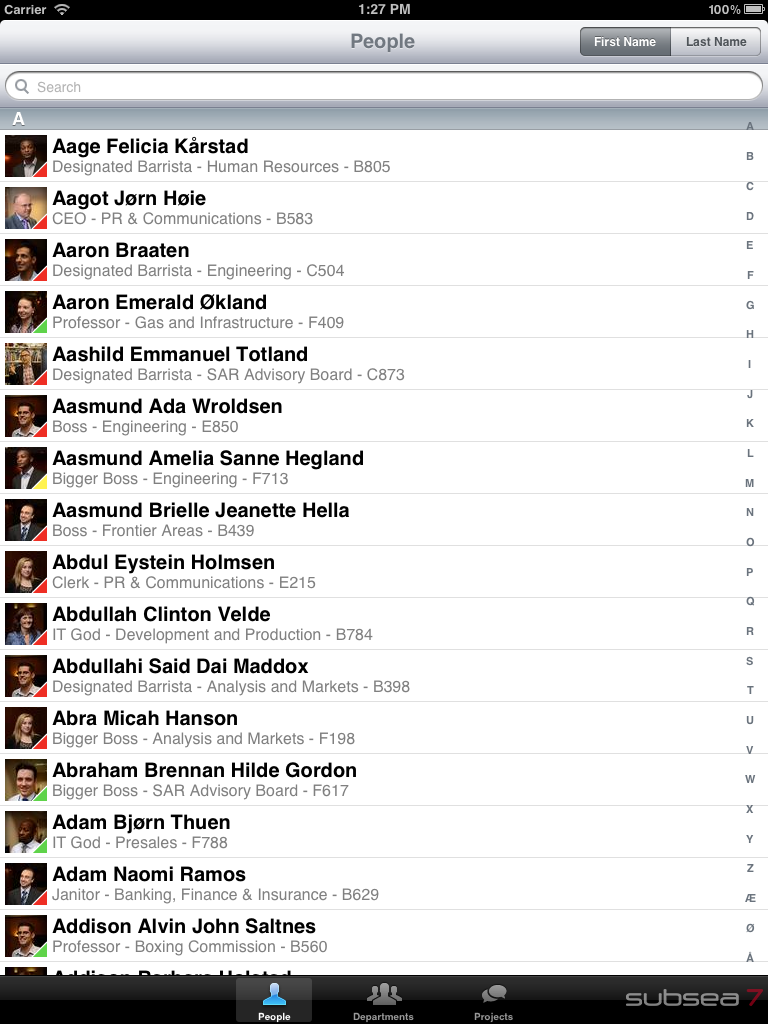
\includegraphics[scale=0.5]{screen_people} }
    \caption{The top level employee list containing all employees.}
    \label{fig:screen_people}
\end{figure}

\subsubsection{Searching an Employee List}

\begin{figure}[H]
    \centerline{ 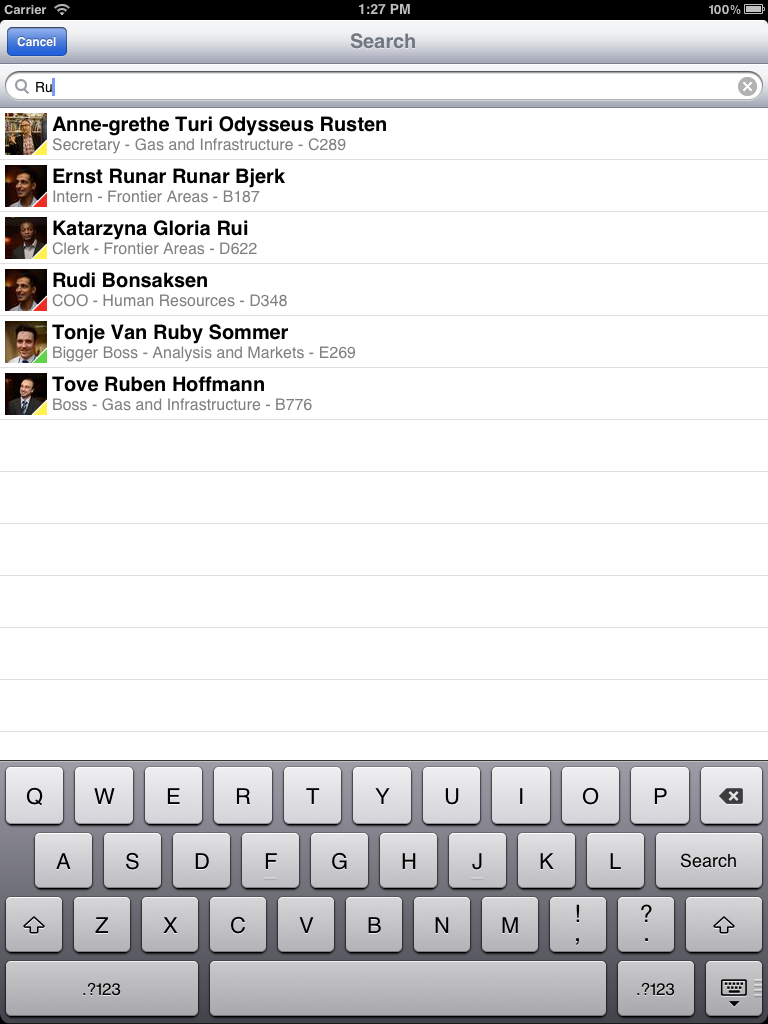
\includegraphics[scale=0.5]{screen_search} }
    \caption{Searching an employee list with the text "Ru".}
    \label{fig:screen_search}
\end{figure}

\subsubsection{Department List}

\begin{figure}[H]
    \centerline{ 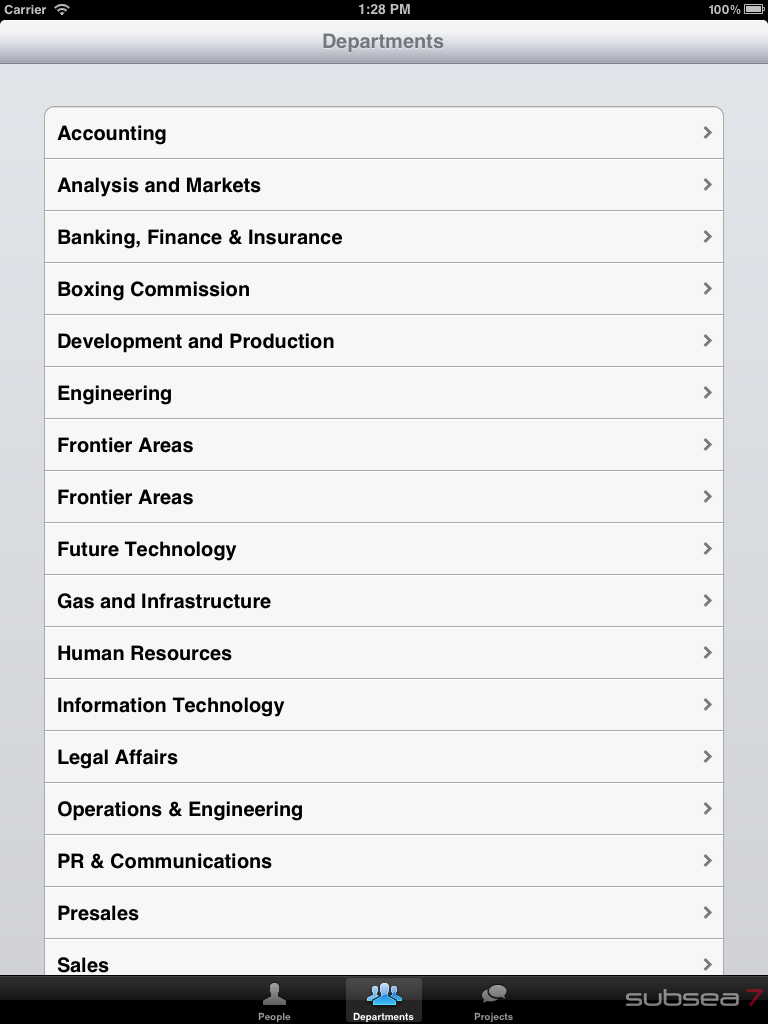
\includegraphics[scale=0.5]{screen_departments} }
    \caption{The top level screen displaying all departments.}
    \label{fig:screen_departments}
\end{figure}

\subsubsection{Employee Profile}

\begin{figure}[H]
    \centerline{ 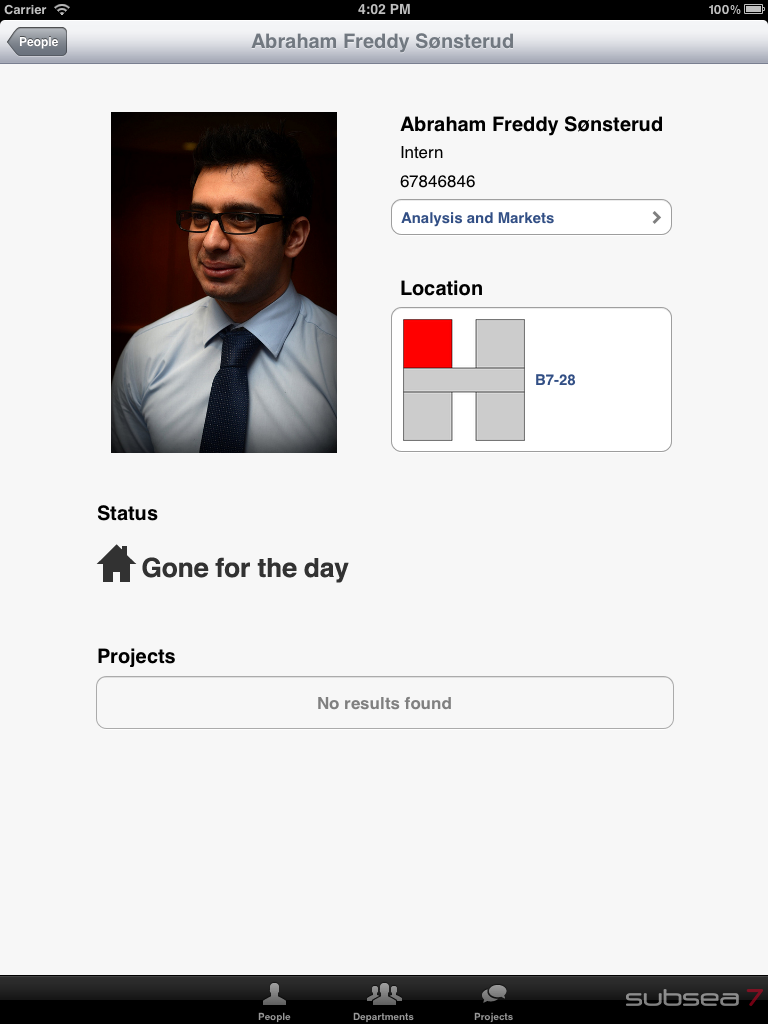
\includegraphics[scale=0.5]{screen_profile} }
    \caption{A profile for an employee.}
    \label{fig:screen_profile}
\end{figure}

\clearpage

\subsection{User Interaction Diagram}

\begin{figure}[H]
    \centerline{ 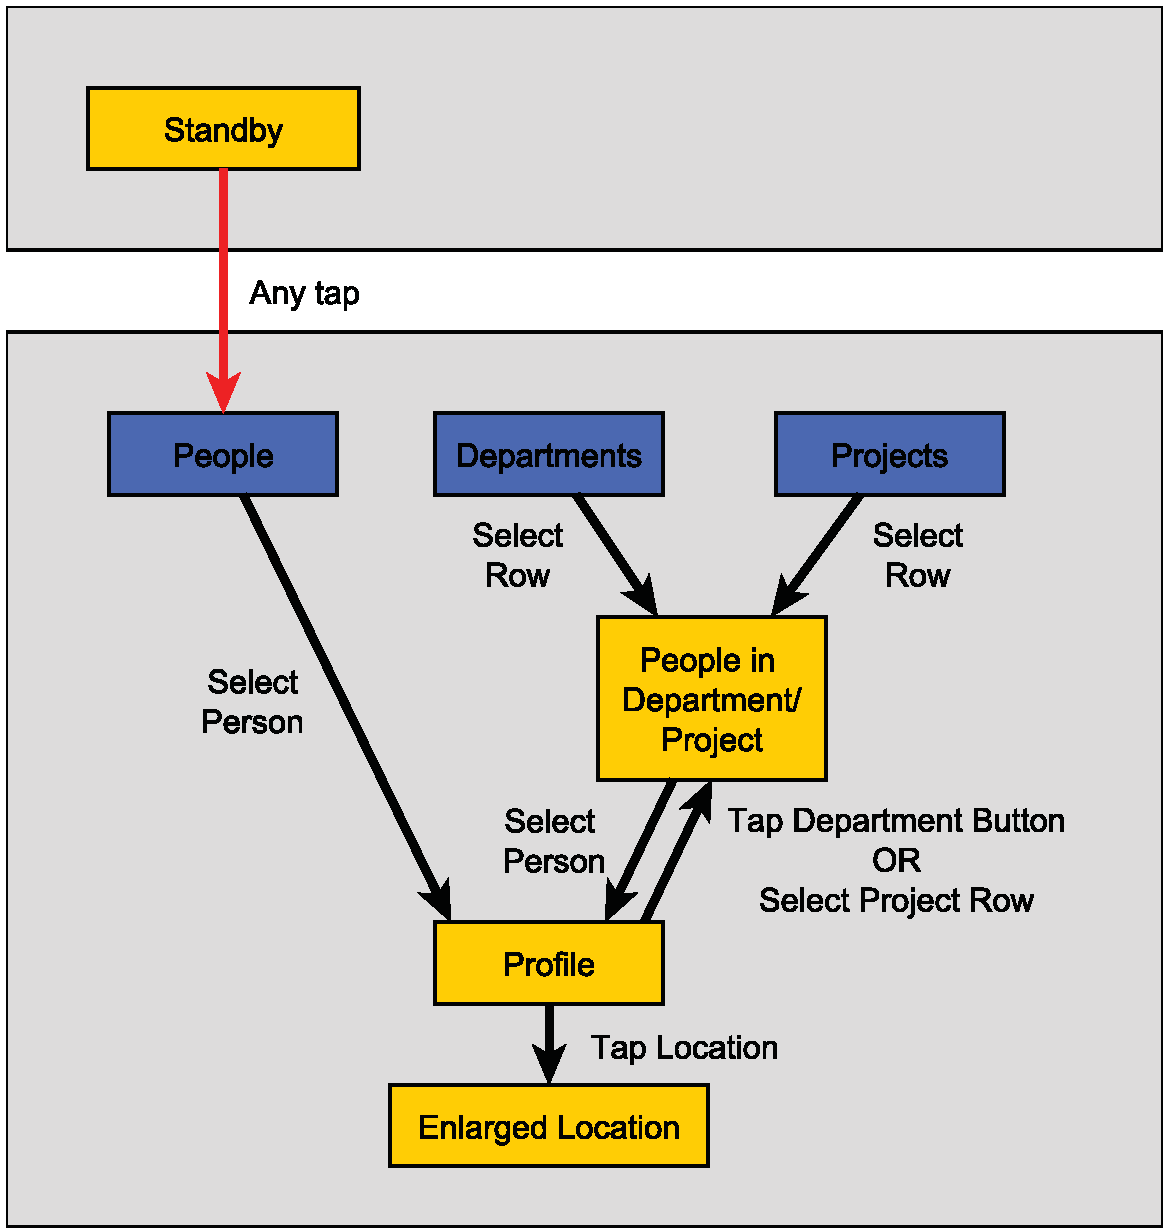
\includegraphics[width=1\textwidth]{interaction_diagram} }
    \caption{Navigation diagram for the user interaction.}
    \label{fig:interaction}
\end{figure}

\fref{fig:interaction} shows the interaction flow for our application.

Small boxes represent a screen in the application. The blue boxes
indicate top level screens when the program is active. Switching to
one of these can be done at any time (except when the location image
is shown in an enlarged version, in which the pop-up has to be closed
first). Doing so will reset the current state.

The two large boxes group the screens, showing if they're used when
the program is user interaction enabled and actively used (lower) or
when inactive (upper).

Arrows indicate a transition from one screen to an other. It is
possible to follow the arrow back to the previous screen. Black arrows
are initiated by users, and the users control when (and if) to go
back. Red arrows are initiated by users, but the application controls
when to go back.

%\subsection{Audio-Visual Presentation}

%The presentation can be found at
%\url{http://www.youtube.com/watch?v=aTGoGxTlfmY}.

\subsection{Think-aloud experiment}

We did a little test of our GUI when we first arrived at Subsea7 at
our final meeting in Stavanger. We needed to test if the user
interface was clearly understandable. For the think-aloud experiment,
the test subject, a woman of age 32, were asked to complete the following tasks:

\begin{description}
\item[Where does "Adam Bjørn Thuen" sit?] She looked at the standby
  screen, quickly tapped it and started reading the names on the list,
  from the top. She found him pretty quickly and tapped his row, and
  could tell us the correct answer: "F788".
\item[What status does "Jørgen Kjær" have?] She spent a little time
  looking around at the screen, but found the back button pretty
  fast. Then she started scrolling down the list. After reaching ``D'' she
  got tired of that, and tapped the search bar. Then she wrote in ``J Ø
  R G E N'', and looked up to see if he was there yet. ``Jørgen Kjær'' had
  been the only result since ``J Ø R'', but she hadn't noticed. She
  tapped his row and could tell us that he was on vacation.
\item[Find someone ``available'' in Jørgen Kjærs' Department.] She
  noted his department "Human Resources" and tapped the "Departments"
  button on the tap bar in the button. Then she found the correct row,
  and tapped that. Then she started tapping the first row, going back
  because the employee was unavailable, tapping the second row, going
  back because the next employee wasn't available either, and so on
  until she reached someone who was available.
\item[Find out where to go for visiting the "Sales" department.] She
  tapped the departments button again, this time selecting
  "Sales". She didn't notice the button that would bring up the
  general location, but selected a few different employees to try
  finding a pattern in their location (there wasn't one because we
  hadn't made any such connection when generating our data). So she
  told us they where sitting all over the place in locations that
  didn't even exists in their building.
\end{description}

So testing with real data would definitely have been a lot better, as
our generated data had a bad effect on the user test -- things didn't
work as our test person was used to. But, we did see some problems
with our user interface that could be improved, and resulting in the
following improvements:

\begin{itemize}
\item We made the status indicator overlays much larger and with much
  stronger colours.
\item We added a disclosure indicator on top of the department button
  (the little arrow), so people would easier understand it was a
  button.
\item We changed the way to display project/department locations, so
  they're just shown in the top no matter what.
\end{itemize}

After implementing the above, we performed the same test again with
real data, albeit with altered names, and it went a lot better. The
new test person understood the coloured triangles, that the department
button was a button, and couldn't miss the location for the
department. The screenshots shown in \aref{sec:gui_ui} are from this
improved version.
